\documentclass[11pt]{article}

    \usepackage[breakable]{tcolorbox}
    \usepackage{parskip} % Stop auto-indenting (to mimic markdown behaviour)
    

    % Basic figure setup, for now with no caption control since it's done
    % automatically by Pandoc (which extracts ![](path) syntax from Markdown).
    \usepackage{graphicx}
    % Maintain compatibility with old templates. Remove in nbconvert 6.0
    \let\Oldincludegraphics\includegraphics
    % Ensure that by default, figures have no caption (until we provide a
    % proper Figure object with a Caption API and a way to capture that
    % in the conversion process - todo).
    \usepackage{caption}
    \DeclareCaptionFormat{nocaption}{}
    \captionsetup{format=nocaption,aboveskip=0pt,belowskip=0pt}

    \usepackage{float}
    \floatplacement{figure}{H} % forces figures to be placed at the correct location
    \usepackage{xcolor} % Allow colors to be defined
    \usepackage{enumerate} % Needed for markdown enumerations to work
    \usepackage{geometry} % Used to adjust the document margins
    \usepackage{amsmath} % Equations
    \usepackage{amssymb} % Equations
    \usepackage{textcomp} % defines textquotesingle
    % Hack from http://tex.stackexchange.com/a/47451/13684:
    \AtBeginDocument{%
        \def\PYZsq{\textquotesingle}% Upright quotes in Pygmentized code
    }
    \usepackage{upquote} % Upright quotes for verbatim code
    \usepackage{eurosym} % defines \euro

    \usepackage{iftex}
    \ifPDFTeX
        \usepackage[T1]{fontenc}
        \IfFileExists{alphabeta.sty}{
              \usepackage{alphabeta}
          }{
              \usepackage[mathletters]{ucs}
              \usepackage[utf8x]{inputenc}
          }
    \else
        \usepackage{fontspec}
        \usepackage{unicode-math}
    \fi

    \usepackage{fancyvrb} % verbatim replacement that allows latex
    \usepackage{grffile} % extends the file name processing of package graphics
                         % to support a larger range
    \makeatletter % fix for old versions of grffile with XeLaTeX
    \@ifpackagelater{grffile}{2019/11/01}
    {
      % Do nothing on new versions
    }
    {
      \def\Gread@@xetex#1{%
        \IfFileExists{"\Gin@base".bb}%
        {\Gread@eps{\Gin@base.bb}}%
        {\Gread@@xetex@aux#1}%
      }
    }
    \makeatother
    \usepackage[Export]{adjustbox} % Used to constrain images to a maximum size
    \adjustboxset{max size={0.9\linewidth}{0.9\paperheight}}

    % The hyperref package gives us a pdf with properly built
    % internal navigation ('pdf bookmarks' for the table of contents,
    % internal cross-reference links, web links for URLs, etc.)
    \usepackage{hyperref}
    % The default LaTeX title has an obnoxious amount of whitespace. By default,
    % titling removes some of it. It also provides customization options.
    \usepackage{titling}
    \usepackage{longtable} % longtable support required by pandoc >1.10
    \usepackage{booktabs}  % table support for pandoc > 1.12.2
    \usepackage{array}     % table support for pandoc >= 2.11.3
    \usepackage{calc}      % table minipage width calculation for pandoc >= 2.11.1
    \usepackage[inline]{enumitem} % IRkernel/repr support (it uses the enumerate* environment)
    \usepackage[normalem]{ulem} % ulem is needed to support strikethroughs (\sout)
                                % normalem makes italics be italics, not underlines
    \usepackage{mathrsfs}
    

    
    % Colors for the hyperref package
    \definecolor{urlcolor}{rgb}{0,.145,.698}
    \definecolor{linkcolor}{rgb}{.71,0.21,0.01}
    \definecolor{citecolor}{rgb}{.12,.54,.11}

    % ANSI colors
    \definecolor{ansi-black}{HTML}{3E424D}
    \definecolor{ansi-black-intense}{HTML}{282C36}
    \definecolor{ansi-red}{HTML}{E75C58}
    \definecolor{ansi-red-intense}{HTML}{B22B31}
    \definecolor{ansi-green}{HTML}{00A250}
    \definecolor{ansi-green-intense}{HTML}{007427}
    \definecolor{ansi-yellow}{HTML}{DDB62B}
    \definecolor{ansi-yellow-intense}{HTML}{B27D12}
    \definecolor{ansi-blue}{HTML}{208FFB}
    \definecolor{ansi-blue-intense}{HTML}{0065CA}
    \definecolor{ansi-magenta}{HTML}{D160C4}
    \definecolor{ansi-magenta-intense}{HTML}{A03196}
    \definecolor{ansi-cyan}{HTML}{60C6C8}
    \definecolor{ansi-cyan-intense}{HTML}{258F8F}
    \definecolor{ansi-white}{HTML}{C5C1B4}
    \definecolor{ansi-white-intense}{HTML}{A1A6B2}
    \definecolor{ansi-default-inverse-fg}{HTML}{FFFFFF}
    \definecolor{ansi-default-inverse-bg}{HTML}{000000}

    % common color for the border for error outputs.
    \definecolor{outerrorbackground}{HTML}{FFDFDF}

    % commands and environments needed by pandoc snippets
    % extracted from the output of `pandoc -s`
    \providecommand{\tightlist}{%
      \setlength{\itemsep}{0pt}\setlength{\parskip}{0pt}}
    \DefineVerbatimEnvironment{Highlighting}{Verbatim}{commandchars=\\\{\}}
    % Add ',fontsize=\small' for more characters per line
    \newenvironment{Shaded}{}{}
    \newcommand{\KeywordTok}[1]{\textcolor[rgb]{0.00,0.44,0.13}{\textbf{{#1}}}}
    \newcommand{\DataTypeTok}[1]{\textcolor[rgb]{0.56,0.13,0.00}{{#1}}}
    \newcommand{\DecValTok}[1]{\textcolor[rgb]{0.25,0.63,0.44}{{#1}}}
    \newcommand{\BaseNTok}[1]{\textcolor[rgb]{0.25,0.63,0.44}{{#1}}}
    \newcommand{\FloatTok}[1]{\textcolor[rgb]{0.25,0.63,0.44}{{#1}}}
    \newcommand{\CharTok}[1]{\textcolor[rgb]{0.25,0.44,0.63}{{#1}}}
    \newcommand{\StringTok}[1]{\textcolor[rgb]{0.25,0.44,0.63}{{#1}}}
    \newcommand{\CommentTok}[1]{\textcolor[rgb]{0.38,0.63,0.69}{\textit{{#1}}}}
    \newcommand{\OtherTok}[1]{\textcolor[rgb]{0.00,0.44,0.13}{{#1}}}
    \newcommand{\AlertTok}[1]{\textcolor[rgb]{1.00,0.00,0.00}{\textbf{{#1}}}}
    \newcommand{\FunctionTok}[1]{\textcolor[rgb]{0.02,0.16,0.49}{{#1}}}
    \newcommand{\RegionMarkerTok}[1]{{#1}}
    \newcommand{\ErrorTok}[1]{\textcolor[rgb]{1.00,0.00,0.00}{\textbf{{#1}}}}
    \newcommand{\NormalTok}[1]{{#1}}

    % Additional commands for more recent versions of Pandoc
    \newcommand{\ConstantTok}[1]{\textcolor[rgb]{0.53,0.00,0.00}{{#1}}}
    \newcommand{\SpecialCharTok}[1]{\textcolor[rgb]{0.25,0.44,0.63}{{#1}}}
    \newcommand{\VerbatimStringTok}[1]{\textcolor[rgb]{0.25,0.44,0.63}{{#1}}}
    \newcommand{\SpecialStringTok}[1]{\textcolor[rgb]{0.73,0.40,0.53}{{#1}}}
    \newcommand{\ImportTok}[1]{{#1}}
    \newcommand{\DocumentationTok}[1]{\textcolor[rgb]{0.73,0.13,0.13}{\textit{{#1}}}}
    \newcommand{\AnnotationTok}[1]{\textcolor[rgb]{0.38,0.63,0.69}{\textbf{\textit{{#1}}}}}
    \newcommand{\CommentVarTok}[1]{\textcolor[rgb]{0.38,0.63,0.69}{\textbf{\textit{{#1}}}}}
    \newcommand{\VariableTok}[1]{\textcolor[rgb]{0.10,0.09,0.49}{{#1}}}
    \newcommand{\ControlFlowTok}[1]{\textcolor[rgb]{0.00,0.44,0.13}{\textbf{{#1}}}}
    \newcommand{\OperatorTok}[1]{\textcolor[rgb]{0.40,0.40,0.40}{{#1}}}
    \newcommand{\BuiltInTok}[1]{{#1}}
    \newcommand{\ExtensionTok}[1]{{#1}}
    \newcommand{\PreprocessorTok}[1]{\textcolor[rgb]{0.74,0.48,0.00}{{#1}}}
    \newcommand{\AttributeTok}[1]{\textcolor[rgb]{0.49,0.56,0.16}{{#1}}}
    \newcommand{\InformationTok}[1]{\textcolor[rgb]{0.38,0.63,0.69}{\textbf{\textit{{#1}}}}}
    \newcommand{\WarningTok}[1]{\textcolor[rgb]{0.38,0.63,0.69}{\textbf{\textit{{#1}}}}}


    % Define a nice break command that doesn't care if a line doesn't already
    % exist.
    \def\br{\hspace*{\fill} \\* }
    % Math Jax compatibility definitions
    \def\gt{>}
    \def\lt{<}
    \let\Oldtex\TeX
    \let\Oldlatex\LaTeX
    \renewcommand{\TeX}{\textrm{\Oldtex}}
    \renewcommand{\LaTeX}{\textrm{\Oldlatex}}
    % Document parameters
    % Document title
    \title{Taller Analisis Algoritmos Dianmicos}
   \author{Santiago Andres Leal Omaña, Santiago Guerrero Vargas} 
    \break
    
    
    
% Pygments definitions
\makeatletter
\def\PY@reset{\let\PY@it=\relax \let\PY@bf=\relax%
    \let\PY@ul=\relax \let\PY@tc=\relax%
    \let\PY@bc=\relax \let\PY@ff=\relax}
\def\PY@tok#1{\csname PY@tok@#1\endcsname}
\def\PY@toks#1+{\ifx\relax#1\empty\else%
    \PY@tok{#1}\expandafter\PY@toks\fi}
\def\PY@do#1{\PY@bc{\PY@tc{\PY@ul{%
    \PY@it{\PY@bf{\PY@ff{#1}}}}}}}
\def\PY#1#2{\PY@reset\PY@toks#1+\relax+\PY@do{#2}}

\@namedef{PY@tok@w}{\def\PY@tc##1{\textcolor[rgb]{0.73,0.73,0.73}{##1}}}
\@namedef{PY@tok@c}{\let\PY@it=\textit\def\PY@tc##1{\textcolor[rgb]{0.24,0.48,0.48}{##1}}}
\@namedef{PY@tok@cp}{\def\PY@tc##1{\textcolor[rgb]{0.61,0.40,0.00}{##1}}}
\@namedef{PY@tok@k}{\let\PY@bf=\textbf\def\PY@tc##1{\textcolor[rgb]{0.00,0.50,0.00}{##1}}}
\@namedef{PY@tok@kp}{\def\PY@tc##1{\textcolor[rgb]{0.00,0.50,0.00}{##1}}}
\@namedef{PY@tok@kt}{\def\PY@tc##1{\textcolor[rgb]{0.69,0.00,0.25}{##1}}}
\@namedef{PY@tok@o}{\def\PY@tc##1{\textcolor[rgb]{0.40,0.40,0.40}{##1}}}
\@namedef{PY@tok@ow}{\let\PY@bf=\textbf\def\PY@tc##1{\textcolor[rgb]{0.67,0.13,1.00}{##1}}}
\@namedef{PY@tok@nb}{\def\PY@tc##1{\textcolor[rgb]{0.00,0.50,0.00}{##1}}}
\@namedef{PY@tok@nf}{\def\PY@tc##1{\textcolor[rgb]{0.00,0.00,1.00}{##1}}}
\@namedef{PY@tok@nc}{\let\PY@bf=\textbf\def\PY@tc##1{\textcolor[rgb]{0.00,0.00,1.00}{##1}}}
\@namedef{PY@tok@nn}{\let\PY@bf=\textbf\def\PY@tc##1{\textcolor[rgb]{0.00,0.00,1.00}{##1}}}
\@namedef{PY@tok@ne}{\let\PY@bf=\textbf\def\PY@tc##1{\textcolor[rgb]{0.80,0.25,0.22}{##1}}}
\@namedef{PY@tok@nv}{\def\PY@tc##1{\textcolor[rgb]{0.10,0.09,0.49}{##1}}}
\@namedef{PY@tok@no}{\def\PY@tc##1{\textcolor[rgb]{0.53,0.00,0.00}{##1}}}
\@namedef{PY@tok@nl}{\def\PY@tc##1{\textcolor[rgb]{0.46,0.46,0.00}{##1}}}
\@namedef{PY@tok@ni}{\let\PY@bf=\textbf\def\PY@tc##1{\textcolor[rgb]{0.44,0.44,0.44}{##1}}}
\@namedef{PY@tok@na}{\def\PY@tc##1{\textcolor[rgb]{0.41,0.47,0.13}{##1}}}
\@namedef{PY@tok@nt}{\let\PY@bf=\textbf\def\PY@tc##1{\textcolor[rgb]{0.00,0.50,0.00}{##1}}}
\@namedef{PY@tok@nd}{\def\PY@tc##1{\textcolor[rgb]{0.67,0.13,1.00}{##1}}}
\@namedef{PY@tok@s}{\def\PY@tc##1{\textcolor[rgb]{0.73,0.13,0.13}{##1}}}
\@namedef{PY@tok@sd}{\let\PY@it=\textit\def\PY@tc##1{\textcolor[rgb]{0.73,0.13,0.13}{##1}}}
\@namedef{PY@tok@si}{\let\PY@bf=\textbf\def\PY@tc##1{\textcolor[rgb]{0.64,0.35,0.47}{##1}}}
\@namedef{PY@tok@se}{\let\PY@bf=\textbf\def\PY@tc##1{\textcolor[rgb]{0.67,0.36,0.12}{##1}}}
\@namedef{PY@tok@sr}{\def\PY@tc##1{\textcolor[rgb]{0.64,0.35,0.47}{##1}}}
\@namedef{PY@tok@ss}{\def\PY@tc##1{\textcolor[rgb]{0.10,0.09,0.49}{##1}}}
\@namedef{PY@tok@sx}{\def\PY@tc##1{\textcolor[rgb]{0.00,0.50,0.00}{##1}}}
\@namedef{PY@tok@m}{\def\PY@tc##1{\textcolor[rgb]{0.40,0.40,0.40}{##1}}}
\@namedef{PY@tok@gh}{\let\PY@bf=\textbf\def\PY@tc##1{\textcolor[rgb]{0.00,0.00,0.50}{##1}}}
\@namedef{PY@tok@gu}{\let\PY@bf=\textbf\def\PY@tc##1{\textcolor[rgb]{0.50,0.00,0.50}{##1}}}
\@namedef{PY@tok@gd}{\def\PY@tc##1{\textcolor[rgb]{0.63,0.00,0.00}{##1}}}
\@namedef{PY@tok@gi}{\def\PY@tc##1{\textcolor[rgb]{0.00,0.52,0.00}{##1}}}
\@namedef{PY@tok@gr}{\def\PY@tc##1{\textcolor[rgb]{0.89,0.00,0.00}{##1}}}
\@namedef{PY@tok@ge}{\let\PY@it=\textit}
\@namedef{PY@tok@gs}{\let\PY@bf=\textbf}
\@namedef{PY@tok@gp}{\let\PY@bf=\textbf\def\PY@tc##1{\textcolor[rgb]{0.00,0.00,0.50}{##1}}}
\@namedef{PY@tok@go}{\def\PY@tc##1{\textcolor[rgb]{0.44,0.44,0.44}{##1}}}
\@namedef{PY@tok@gt}{\def\PY@tc##1{\textcolor[rgb]{0.00,0.27,0.87}{##1}}}
\@namedef{PY@tok@err}{\def\PY@bc##1{{\setlength{\fboxsep}{\string -\fboxrule}\fcolorbox[rgb]{1.00,0.00,0.00}{1,1,1}{\strut ##1}}}}
\@namedef{PY@tok@kc}{\let\PY@bf=\textbf\def\PY@tc##1{\textcolor[rgb]{0.00,0.50,0.00}{##1}}}
\@namedef{PY@tok@kd}{\let\PY@bf=\textbf\def\PY@tc##1{\textcolor[rgb]{0.00,0.50,0.00}{##1}}}
\@namedef{PY@tok@kn}{\let\PY@bf=\textbf\def\PY@tc##1{\textcolor[rgb]{0.00,0.50,0.00}{##1}}}
\@namedef{PY@tok@kr}{\let\PY@bf=\textbf\def\PY@tc##1{\textcolor[rgb]{0.00,0.50,0.00}{##1}}}
\@namedef{PY@tok@bp}{\def\PY@tc##1{\textcolor[rgb]{0.00,0.50,0.00}{##1}}}
\@namedef{PY@tok@fm}{\def\PY@tc##1{\textcolor[rgb]{0.00,0.00,1.00}{##1}}}
\@namedef{PY@tok@vc}{\def\PY@tc##1{\textcolor[rgb]{0.10,0.09,0.49}{##1}}}
\@namedef{PY@tok@vg}{\def\PY@tc##1{\textcolor[rgb]{0.10,0.09,0.49}{##1}}}
\@namedef{PY@tok@vi}{\def\PY@tc##1{\textcolor[rgb]{0.10,0.09,0.49}{##1}}}
\@namedef{PY@tok@vm}{\def\PY@tc##1{\textcolor[rgb]{0.10,0.09,0.49}{##1}}}
\@namedef{PY@tok@sa}{\def\PY@tc##1{\textcolor[rgb]{0.73,0.13,0.13}{##1}}}
\@namedef{PY@tok@sb}{\def\PY@tc##1{\textcolor[rgb]{0.73,0.13,0.13}{##1}}}
\@namedef{PY@tok@sc}{\def\PY@tc##1{\textcolor[rgb]{0.73,0.13,0.13}{##1}}}
\@namedef{PY@tok@dl}{\def\PY@tc##1{\textcolor[rgb]{0.73,0.13,0.13}{##1}}}
\@namedef{PY@tok@s2}{\def\PY@tc##1{\textcolor[rgb]{0.73,0.13,0.13}{##1}}}
\@namedef{PY@tok@sh}{\def\PY@tc##1{\textcolor[rgb]{0.73,0.13,0.13}{##1}}}
\@namedef{PY@tok@s1}{\def\PY@tc##1{\textcolor[rgb]{0.73,0.13,0.13}{##1}}}
\@namedef{PY@tok@mb}{\def\PY@tc##1{\textcolor[rgb]{0.40,0.40,0.40}{##1}}}
\@namedef{PY@tok@mf}{\def\PY@tc##1{\textcolor[rgb]{0.40,0.40,0.40}{##1}}}
\@namedef{PY@tok@mh}{\def\PY@tc##1{\textcolor[rgb]{0.40,0.40,0.40}{##1}}}
\@namedef{PY@tok@mi}{\def\PY@tc##1{\textcolor[rgb]{0.40,0.40,0.40}{##1}}}
\@namedef{PY@tok@il}{\def\PY@tc##1{\textcolor[rgb]{0.40,0.40,0.40}{##1}}}
\@namedef{PY@tok@mo}{\def\PY@tc##1{\textcolor[rgb]{0.40,0.40,0.40}{##1}}}
\@namedef{PY@tok@ch}{\let\PY@it=\textit\def\PY@tc##1{\textcolor[rgb]{0.24,0.48,0.48}{##1}}}
\@namedef{PY@tok@cm}{\let\PY@it=\textit\def\PY@tc##1{\textcolor[rgb]{0.24,0.48,0.48}{##1}}}
\@namedef{PY@tok@cpf}{\let\PY@it=\textit\def\PY@tc##1{\textcolor[rgb]{0.24,0.48,0.48}{##1}}}
\@namedef{PY@tok@c1}{\let\PY@it=\textit\def\PY@tc##1{\textcolor[rgb]{0.24,0.48,0.48}{##1}}}
\@namedef{PY@tok@cs}{\let\PY@it=\textit\def\PY@tc##1{\textcolor[rgb]{0.24,0.48,0.48}{##1}}}

\def\PYZbs{\char`\\}
\def\PYZus{\char`\_}
\def\PYZob{\char`\{}
\def\PYZcb{\char`\}}
\def\PYZca{\char`\^}
\def\PYZam{\char`\&}
\def\PYZlt{\char`\<}
\def\PYZgt{\char`\>}
\def\PYZsh{\char`\#}
\def\PYZpc{\char`\%}
\def\PYZdl{\char`\$}
\def\PYZhy{\char`\-}
\def\PYZsq{\char`\'}
\def\PYZdq{\char`\"}
\def\PYZti{\char`\~}
% for compatibility with earlier versions
\def\PYZat{@}
\def\PYZlb{[}
\def\PYZrb{]}
\makeatother


    % For linebreaks inside Verbatim environment from package fancyvrb.
    \makeatletter
        \newbox\Wrappedcontinuationbox
        \newbox\Wrappedvisiblespacebox
        \newcommand*\Wrappedvisiblespace {\textcolor{red}{\textvisiblespace}}
        \newcommand*\Wrappedcontinuationsymbol {\textcolor{red}{\llap{\tiny$\m@th\hookrightarrow$}}}
        \newcommand*\Wrappedcontinuationindent {3ex }
        \newcommand*\Wrappedafterbreak {\kern\Wrappedcontinuationindent\copy\Wrappedcontinuationbox}
        % Take advantage of the already applied Pygments mark-up to insert
        % potential linebreaks for TeX processing.
        %        {, <, #, %, $, ' and ": go to next line.
        %        _, }, ^, &, >, - and ~: stay at end of broken line.
        % Use of \textquotesingle for straight quote.
        \newcommand*\Wrappedbreaksatspecials {%
            \def\PYGZus{\discretionary{\char`\_}{\Wrappedafterbreak}{\char`\_}}%
            \def\PYGZob{\discretionary{}{\Wrappedafterbreak\char`\{}{\char`\{}}%
            \def\PYGZcb{\discretionary{\char`\}}{\Wrappedafterbreak}{\char`\}}}%
            \def\PYGZca{\discretionary{\char`\^}{\Wrappedafterbreak}{\char`\^}}%
            \def\PYGZam{\discretionary{\char`\&}{\Wrappedafterbreak}{\char`\&}}%
            \def\PYGZlt{\discretionary{}{\Wrappedafterbreak\char`\<}{\char`\<}}%
            \def\PYGZgt{\discretionary{\char`\>}{\Wrappedafterbreak}{\char`\>}}%
            \def\PYGZsh{\discretionary{}{\Wrappedafterbreak\char`\#}{\char`\#}}%
            \def\PYGZpc{\discretionary{}{\Wrappedafterbreak\char`\%}{\char`\%}}%
            \def\PYGZdl{\discretionary{}{\Wrappedafterbreak\char`\$}{\char`\$}}%
            \def\PYGZhy{\discretionary{\char`\-}{\Wrappedafterbreak}{\char`\-}}%
            \def\PYGZsq{\discretionary{}{\Wrappedafterbreak\textquotesingle}{\textquotesingle}}%
            \def\PYGZdq{\discretionary{}{\Wrappedafterbreak\char`\"}{\char`\"}}%
            \def\PYGZti{\discretionary{\char`\~}{\Wrappedafterbreak}{\char`\~}}%
        }
        % Some characters . , ; ? ! / are not pygmentized.
        % This macro makes them "active" and they will insert potential linebreaks
        \newcommand*\Wrappedbreaksatpunct {%
            \lccode`\~`\.\lowercase{\def~}{\discretionary{\hbox{\char`\.}}{\Wrappedafterbreak}{\hbox{\char`\.}}}%
            \lccode`\~`\,\lowercase{\def~}{\discretionary{\hbox{\char`\,}}{\Wrappedafterbreak}{\hbox{\char`\,}}}%
            \lccode`\~`\;\lowercase{\def~}{\discretionary{\hbox{\char`\;}}{\Wrappedafterbreak}{\hbox{\char`\;}}}%
            \lccode`\~`\:\lowercase{\def~}{\discretionary{\hbox{\char`\:}}{\Wrappedafterbreak}{\hbox{\char`\:}}}%
            \lccode`\~`\?\lowercase{\def~}{\discretionary{\hbox{\char`\?}}{\Wrappedafterbreak}{\hbox{\char`\?}}}%
            \lccode`\~`\!\lowercase{\def~}{\discretionary{\hbox{\char`\!}}{\Wrappedafterbreak}{\hbox{\char`\!}}}%
            \lccode`\~`\/\lowercase{\def~}{\discretionary{\hbox{\char`\/}}{\Wrappedafterbreak}{\hbox{\char`\/}}}%
            \catcode`\.\active
            \catcode`\,\active
            \catcode`\;\active
            \catcode`\:\active
            \catcode`\?\active
            \catcode`\!\active
            \catcode`\/\active
            \lccode`\~`\~
        }
    \makeatother

    \let\OriginalVerbatim=\Verbatim
    \makeatletter
    \renewcommand{\Verbatim}[1][1]{%
        %\parskip\z@skip
        \sbox\Wrappedcontinuationbox {\Wrappedcontinuationsymbol}%
        \sbox\Wrappedvisiblespacebox {\FV@SetupFont\Wrappedvisiblespace}%
        \def\FancyVerbFormatLine ##1{\hsize\linewidth
            \vtop{\raggedright\hyphenpenalty\z@\exhyphenpenalty\z@
                \doublehyphendemerits\z@\finalhyphendemerits\z@
                \strut ##1\strut}%
        }%
        % If the linebreak is at a space, the latter will be displayed as visible
        % space at end of first line, and a continuation symbol starts next line.
        % Stretch/shrink are however usually zero for typewriter font.
        \def\FV@Space {%
            \nobreak\hskip\z@ plus\fontdimen3\font minus\fontdimen4\font
            \discretionary{\copy\Wrappedvisiblespacebox}{\Wrappedafterbreak}
            {\kern\fontdimen2\font}%
        }%

        % Allow breaks at special characters using \PYG... macros.
        \Wrappedbreaksatspecials
        % Breaks at punctuation characters . , ; ? ! and / need catcode=\active
        \OriginalVerbatim[#1,codes*=\Wrappedbreaksatpunct]%
    }
    \makeatother

    % Exact colors from NB
    \definecolor{incolor}{HTML}{303F9F}
    \definecolor{outcolor}{HTML}{D84315}
    \definecolor{cellborder}{HTML}{CFCFCF}
    \definecolor{cellbackground}{HTML}{F7F7F7}

    % prompt
    \makeatletter
    \newcommand{\boxspacing}{\kern\kvtcb@left@rule\kern\kvtcb@boxsep}
    \makeatother
    \newcommand{\prompt}[4]{
        {\ttfamily\llap{{\color{#2}[#3]:\hspace{3pt}#4}}\vspace{-\baselineskip}}
    }
    

    
    % Prevent overflowing lines due to hard-to-break entities
    \sloppy
    % Setup hyperref package
    \hypersetup{
      breaklinks=true,  % so long urls are correctly broken across lines
      colorlinks=true,
      urlcolor=urlcolor,
      linkcolor=linkcolor,
      citecolor=citecolor,
      }
    % Slightly bigger margins than the latex defaults
    
    \geometry{verbose,tmargin=1in,bmargin=1in,lmargin=1in,rmargin=1in}
    
    

\begin{document}
    
    \maketitle

    \hypertarget{parte-1}{%
\section{Parte 1}\label{parte-1}}

\hypertarget{analisis-y-diseuxf1o-del-problema}{%
\subsection{Analisis y diseño del
problema}\label{analisis-y-diseuxf1o-del-problema}}

\hypertarget{analisis}{%
\subsubsection{Analisis}\label{analisis}}

El problema para resolver es encontrar la subsecuencia contigua en una
secuencia de números reales que produce el mayor producto acumulado en
comparación al resto de la secuencia. Es decir, se debe buscar una
subsecuencia de la secuencia original, tal que, al multiplicar todos sus
elementos, se obtiene el producto máximo en comparación con todas las
demás subsecuencias.

Este problema se puede abordar mediante el uso de un algoritmo eficiente
que recorra la secuencia y calcule el producto acumulado de cada
subsecuencia, para luego compararlas y encontrar la subsecuencia con el
mayor producto. Sin embargo, debido a que hay un número infinito de
subsecuencias posibles en una secuencia de longitud n, se necesitará un
enfoque más eficiente para resolver este problema.

\hypertarget{diseuxf1o}{%
\subsubsection{Diseño}\label{diseuxf1o}}

Entrada: Una secuencia de números reales de longitud n.

Salida: Una subsecuencia con el producto mayor.

\hypertarget{objetivo}{%
\subsubsection{Objetivo}\label{objetivo}}

Escribir tres algoritmos (evidente recursivo, memorizado y bottom-up)
asociados a un diseño de un problema que se puede resolver, usando la
estrategia de programación dinámica.

\hypertarget{subsecuencia-de-producto-muxe1xima}{%
\subsubsection{Subsecuencia de producto
máxima}\label{subsecuencia-de-producto-muxe1xima}}

El desarrollo del taller consistirá en analizar tres algoritmos
asociados al problema de encontrar para una secuencia de elementos X =
⟨x1, . . . , xn⟩, xi ∈ R la subsecuencia de elementos contiguos cuyo
producto es máximo.

Por ejemplo, para la subsecuencia ejemplo X = ⟨−7, 12, −7, 0, 14, −7,
5⟩, la subsecuencia contigua de elementos contiguos cuyo producto es
máximo es X{[}1 : 3{]}

\pagebreak
\hypertarget{parte-2}{%
\section{Parte 2}\label{parte-2}}

A continuacion se muestran los 3 algortimos realizados para la solución
de nuestro problema.

\hypertarget{recursivo}{%
\subsection{Recursivo:}\label{recursivo}}

\\

Este algortimo evalua un intervalo incial, que va desde el incio de la
secuencia incial, y en cada llamado iterativo va recortando el intervalo
a usar, posteriormente se compara cada llamado recursivo en busqueda por
el que posea el mayor valor (producto) y este es el que se retorna.

    \begin{tcolorbox}[breakable, size=fbox, boxrule=1pt, pad at break*=1mm,colback=cellbackground, colframe=cellborder]
\prompt{In}{incolor}{ }{\boxspacing}
\begin{Verbatim}[commandchars=\\\{\}]
\PY{n}{FUNCTION} \PY{n}{rec}\PY{p}{(}\PY{n}{seq}\PY{p}{)}
    \PY{n}{SET} \PY{n}{val}\PY{p}{,}\PY{n}{x}\PY{p}{,}\PY{n}{y} \PY{n}{to} \PY{n}{Rec\PYZus{}2}\PY{p}{(}\PY{n}{seq}\PY{p}{,}\PY{l+m+mi}{0}\PY{p}{,}\PY{n}{length} \PY{n}{of} \PY{n}{seq} \PY{o}{\PYZhy{}} \PY{l+m+mi}{1}\PY{p}{)}
    \PY{n}{RETURN} \PY{n}{subsequence} \PY{k+kn}{from} \PY{n+nn}{seq}\PY{p}{[}\PY{n}{x}\PY{p}{]} \PY{n}{to} \PY{n}{seq}\PY{p}{[}\PY{n}{y}\PY{o}{+}\PY{l+m+mi}{1}\PY{p}{]}

\PY{n}{FUNCTION} \PY{n}{Rec\PYZus{}2}\PY{p}{(}\PY{n}{sec}\PY{p}{,}\PY{n}{i}\PY{p}{,}\PY{n}{j}\PY{p}{)}
    \PY{n}{IF} \PY{n}{i} \PY{o+ow}{is} \PY{n}{equal} \PY{n}{to} \PY{n}{j}
        \PY{n}{RETURN} \PY{n}{sec}\PY{p}{[}\PY{n}{i}\PY{p}{]}\PY{p}{,}\PY{n}{i}\PY{p}{,}\PY{n}{j}
    \PY{n}{ENDIF}
    \PY{n}{SET} \PY{n}{max\PYZus{}product} \PY{n}{to} \PY{l+m+mi}{1}
    \PY{n}{FOR} \PY{n}{k} \PY{n}{FROM} \PY{n}{i} \PY{n}{to} \PY{n}{j}\PY{o}{+}\PY{l+m+mi}{1}
        \PY{n}{max\PYZus{}product} \PY{o}{=} \PY{n}{max\PYZus{}product} \PY{o}{*} \PY{n}{sec}\PY{p}{[}\PY{n}{k}\PY{p}{]}
    \PY{n}{ENDFOR}
    \PY{n}{SET} \PY{n}{t1}\PY{p}{,}\PY{n}{t2}\PY{p}{,}\PY{n}{t3} \PY{n}{to} \PY{n}{Rec\PYZus{}2}\PY{p}{(}\PY{n}{sec}\PY{p}{,}\PY{n}{i}\PY{p}{,}\PY{n}{j}\PY{o}{\PYZhy{}}\PY{l+m+mi}{1}\PY{p}{)}
    \PY{n}{SET} \PY{n}{t4}\PY{p}{,}\PY{n}{t5}\PY{p}{,}\PY{n}{t6} \PY{n}{to} \PY{n}{Rec\PYZus{}2}\PY{p}{(}\PY{n}{sec}\PY{p}{,}\PY{n}{i}\PY{o}{+}\PY{l+m+mi}{1}\PY{p}{,}\PY{n}{j}\PY{p}{)}
    \PY{n}{IF} \PY{n}{max\PYZus{}product} \PY{o+ow}{is} \PY{n}{greater} \PY{n}{than} \PY{n}{t1} \PY{o+ow}{and} \PY{n}{max\PYZus{}product} \PY{o+ow}{is} \PY{n}{greater} \PY{n}{than} \PY{n}{t4}
        \PY{n}{RETURN} \PY{n}{max\PYZus{}product}\PY{p}{,}\PY{n}{i}\PY{p}{,}\PY{n}{j}
    \PY{n}{ELSEIF} \PY{n}{t1} \PY{o+ow}{is} \PY{n}{greater} \PY{n}{than} \PY{n}{max\PYZus{}product} \PY{o+ow}{and} \PY{n}{t1} \PY{o+ow}{is} \PY{n}{greater} \PY{n}{than} \PY{n}{t4}
        \PY{n}{RETURN} \PY{n}{t1}\PY{p}{,}\PY{n}{t2}\PY{p}{,}\PY{n}{t3}
    \PY{n}{ELSE}
        \PY{n}{RETURN} \PY{n}{t4}\PY{p}{,}\PY{n}{t5}\PY{p}{,}\PY{n}{t6}
    \PY{n}{ENDIF}
\end{Verbatim}
\end{tcolorbox}

    \hypertarget{complejidad}{%
\subsubsection{Complejidad}\label{complejidad}}
\\
Para poder definir la complejidad, se usa el teorema maestro para
calcular el Big\_O del algoritmo.

\(T(n) = 2T(n-1) + O(1)\)

Esta ecuacion puede ser evaluada de igual manera que el algoritmo
recursivo de fibonnaci, entonces, podemos definir la complejidad en
\(O(2^n)\), la razón por la que es \(O(2^n)\) se debe a que en cada
llamada recursiva, se dividen los elementos en dos subsecuencias, lo que
implica que hay un máximo de \(2^n\) posibles subsecuencias. Además,
como se realiza una multiplicación para cada subsecuencia, la
complejidad de tiempo real total es de \(O(n * 2^n)\), lo que significa
que el algoritmo no es práctico para tamaños de entrada grandes.
\hypertarget{Invariante}{%
\subsubsection{Invariante}\label{complejidad}} \\



Se busca encontrar el intervalo interno con el producto maximo, dentro
de la secuencia dada.

\begin{itemize}
\tightlist
\item
  \textbf{Inicio:} Se sabe que el producto maximo existe dentro de la
  secuencia, por lo que se inicia buscando dentro de toda la secuencia
  desde la posicion 0 y la ultima posición.
\item
  \textbf{Avance:} Como puede que la secuencia completa no sea el
  producto maximo de la misma, se vuelve a llamar la recursion corriendo
  ambos indices, el inicio se mueve hacia la derecha y el final hacia la
  izquierda.
\item
  \textbf{Final:} Cuando la secuencia en la que se esta buscando
  corresponde a un solo elemento se detiene la recursion y se retorna el
  valor que existe en esa secuencia
\end{itemize}

\hypertarget{Top-Bottom }{%
\subsection{Top-Bottom}\label{recursivo}}
\\
Top-Bottom (Memorizado recursivo) En este algoritmo se usa matriz para
poder memorizar el producto posible de cada intervalo que existe, por lo
que en cada llamado recursivo verificamos si el producto que deseamos
obtener ya fue calculado, y de lo contrario se calcula el producto
dentro de ese intervalo.

    \begin{tcolorbox}[breakable, size=fbox, boxrule=1pt, pad at break*=1mm,colback=cellbackground, colframe=cellborder]
\prompt{In}{incolor}{ }{\boxspacing}
\begin{Verbatim}[commandchars=\\\{\}]
\PY{n}{FUNCTION} \PY{n}{MemorizadoRecursivo2}\PY{p}{(}\PY{n}{sec}\PY{p}{,}\PY{n}{i}\PY{p}{,}\PY{n}{j}\PY{p}{,}\PY{n}{M}\PY{p}{)}
    \PY{n}{IF} \PY{n}{i} \PY{o+ow}{is} \PY{n}{equal} \PY{n}{to} \PY{n}{j}
        \PY{n}{M}\PY{p}{[}\PY{n}{i}\PY{p}{]}\PY{p}{[}\PY{n}{j}\PY{p}{]} \PY{o}{=} \PY{n}{sec}\PY{p}{[}\PY{n}{i}\PY{p}{]}
        \PY{n}{RETURN} \PY{n}{sec}\PY{p}{[}\PY{n}{i}\PY{p}{]}\PY{p}{,}\PY{n}{i}\PY{p}{,}\PY{n}{j}
    \PY{n}{ENDIF}
    \PY{n}{IF} \PY{n}{M}\PY{p}{[}\PY{n}{i}\PY{p}{]}\PY{p}{[}\PY{n}{j}\PY{p}{]} \PY{o+ow}{is} \PY{n}{greater} \PY{n}{than} \PY{n}{negative} \PY{n}{infinity}
        \PY{n}{RETURN} \PY{n}{M}\PY{p}{[}\PY{n}{i}\PY{p}{]}\PY{p}{[}\PY{n}{j}\PY{p}{]}\PY{p}{,}\PY{n}{i}\PY{p}{,}\PY{n}{j}
    \PY{n}{ENDIF}
    \PY{n}{SET} \PY{n}{max\PYZus{}product} \PY{n}{to} \PY{l+m+mi}{1}
    \PY{n}{FOR} \PY{n}{k} \PY{n}{FROM} \PY{n}{i} \PY{n}{to} \PY{n}{j}\PY{o}{+}\PY{l+m+mi}{1}
        \PY{n}{max\PYZus{}product} \PY{o}{=} \PY{n}{max\PYZus{}product} \PY{o}{*} \PY{n}{sec}\PY{p}{[}\PY{n}{k}\PY{p}{]}
    \PY{n}{ENDFOR}
    \PY{n}{M}\PY{p}{[}\PY{n}{i}\PY{p}{]}\PY{p}{[}\PY{n}{j}\PY{p}{]} \PY{o}{=} \PY{n}{max\PYZus{}product}
    \PY{n}{CALL} \PY{n}{MemorizadoRecursivo2}\PY{p}{(}\PY{n}{sec}\PY{p}{,}\PY{n}{i}\PY{p}{,}\PY{n}{j}\PY{o}{\PYZhy{}}\PY{l+m+mi}{1}\PY{p}{,}\PY{n}{M}\PY{p}{)}
    \PY{n}{CALL} \PY{n}{MemorizadoRecursivo2}\PY{p}{(}\PY{n}{sec}\PY{p}{,}\PY{n}{i}\PY{o}{+}\PY{l+m+mi}{1}\PY{p}{,}\PY{n}{j}\PY{p}{,}\PY{n}{M}\PY{p}{)}
    \PY{n}{RETURN} \PY{n}{M}

\PY{n}{FUNCTION} \PY{n}{subSequence}\PY{p}{(}\PY{n}{X}\PY{p}{,} \PY{n}{memo}\PY{p}{)}
    \PY{n}{SET} \PY{n}{max\PYZus{}val} \PY{n}{to} \PY{n}{maximum} \PY{n}{value} \PY{o+ow}{in} \PY{n}{memo}
    \PY{n}{SET} \PY{n}{i} \PY{n}{to} \PY{l+m+mi}{0} \PY{o+ow}{and} \PY{n}{j} \PY{n}{to} \PY{n}{length} \PY{n}{of} \PY{n}{X} \PY{o}{\PYZhy{}} \PY{l+m+mi}{1}
    \PY{n}{FOR} \PY{n}{x} \PY{n}{FROM} \PY{l+m+mi}{0} \PY{n}{to} \PY{n}{length} \PY{n}{of} \PY{n}{X}
        \PY{n}{FOR} \PY{n}{y} \PY{n}{FROM} \PY{n}{x} \PY{n}{to} \PY{n}{length} \PY{n}{of} \PY{n}{X}
            \PY{n}{IF} \PY{n}{memo}\PY{p}{[}\PY{n}{x}\PY{p}{]}\PY{p}{[}\PY{n}{y}\PY{p}{]} \PY{o+ow}{is} \PY{n}{equal} \PY{n}{to} \PY{n}{max\PYZus{}val}
                \PY{n}{SET} \PY{n}{i} \PY{n}{to} \PY{n}{x} \PY{o+ow}{and} \PY{n}{j} \PY{n}{to} \PY{n}{y}
                \PY{n}{BREAK}
            \PY{n}{ENDIF}
        \PY{n}{ENDFOR}
    \PY{n}{ENDFOR}
    \PY{n}{RETURN} \PY{n}{subsequence} \PY{k+kn}{from} \PY{n+nn}{X}\PY{p}{[}\PY{n}{i}\PY{p}{]} \PY{n}{to} \PY{n}{X}\PY{p}{[}\PY{n}{j}\PY{o}{+}\PY{l+m+mi}{1}\PY{p}{]}

\PY{n}{FUNCTION} \PY{n}{rec}\PY{p}{(}\PY{n}{seq}\PY{p}{)}
    \PY{n}{SET} \PY{n}{M} \PY{k}{as} \PY{n}{a} \PY{n}{matrix} \PY{k}{with} \PY{n}{dimensions} \PY{p}{(}\PY{n}{length} \PY{n}{of} \PY{n}{seq}\PY{p}{)} \PY{n}{x} \PY{p}{(}\PY{n}{length} \PY{n}{of} \PY{n}{seq}\PY{p}{)} \PY{k}{with} \PY{n+nb}{all} \PY{n}{values} \PY{n+nb}{set} \PY{n}{to} \PY{n}{negative} \PY{n}{infinity}\PY{o}{.}
    \PY{n}{CALL} \PY{n}{MemorizadoRecursivo2}\PY{p}{(}\PY{n}{seq}\PY{p}{,}\PY{l+m+mi}{0}\PY{p}{,}\PY{n}{length} \PY{n}{of} \PY{n}{M} \PY{o}{\PYZhy{}} \PY{l+m+mi}{1}\PY{p}{,}\PY{n}{M}\PY{p}{)}
    \PY{n}{RETURN} \PY{n}{subSequence}\PY{p}{(}\PY{n}{seq}\PY{p}{,} \PY{n}{M}\PY{p}{)}
\end{Verbatim}
\end{tcolorbox}

\hypertarget{complejidad}{%
\subsubsection{Complejidad}\label{complejidad}}
\\

La complejidad del algoritmo se puede analizar utilizando el Teorema
Maestro, que se aplica a las funciones recursivas que se dividen en
subproblemas de tamaño \(a\), que se resuelven recursivamente, y luego
se combinan en una solución de tamaño \(n\).

En este caso, el algoritmo recursivo divide el problema original en dos
subproblemas de tamaño \(n-1\), lo que implica que \(a\) es igual a 1.
El costo de combinar las soluciones de los subproblemas es constante, ya
que solo se realiza una multiplicación y una comparación. Por lo tanto,
\(b\) es igual a 1.

La complejidad del algoritmo está determinada por el costo de resolver
cada subproblema, que en este caso es proporcional al tamaño del
subproblema. En cada llamada recursiva, el tamaño del subproblema
disminuye en 1, lo que significa que la complejidad del algoritmo está
dada por:

\(T(n) = 2T(n-1) + O(n)\)

Donde \(2T(n-1)\) representa el costo de resolver dos subproblemas de
tamaño \(n-1\), y \(O(n)\) es el costo de combinar las soluciones de los
subproblemas.

Según el Teorema Maestro, la complejidad del algoritmo se puede expresar
como:

\(T(n) = O(n^log(a,b))\)

En este caso, \(a\) es igual a 1 y \(b\) es igual a 2, lo que significa
que \(log(a,b)\) es igual a 0. Por lo tanto, la complejidad del
algoritmo es:

\(T(n) = O(n^0 * log(n)) = O(log(n))\)

Sin embargo, como se realiza una multiplicación en cada iteración del
bucle ``for'', la complejidad real del algoritmo es cercana a
\(n log(n)\).

\hypertarget{invariante}{%
\subsubsection{Invariante}\label{invariante}}\\

La invariante del código es que en cada llamada recursiva, la función
MemorizadoRecursivo2() calcula el producto máximo de la subsecuencia de
la secuencia sec desde el índice i hasta el índice j y almacena el
resultado en la matriz M. Luego, la función llama a sí misma
recursivamente para calcular los productos máximos de las subsecuencias
más cortas y actualiza la matriz M con los resultados. Finalmente, la
función devuelve la matriz M actualizada.

\begin{itemize}
\tightlist
\item
  \textbf{Inicio:} La matriz M está inicializada con todos sus valores
  establecidos en float(`-inf'), lo que indica que no se han calculado
  los productos máximos para ninguna subsecuencia de la secuencia dada.
\item
  \textbf{Avance:} Ocurre en cada llamada recursiva de la función
  MemorizadoRecursivo2(). La función calcula el producto máximo de la
  subsecuencia de la secuencia sec desde el índice i hasta el índice j,
  almacena el resultado en la matriz M y llama a sí misma recursivamente
  para calcular los productos máximos de las subsecuencias más cortas.
\item
  \textbf{Final:} Cuando la función llega a la condición base de la
  recursión, es decir, cuando el índice de inicio i es igual al índice
  de finalización j, la función asigna el valor de la secuencia a la
  matriz M. Luego, la función comprueba si el valor de la matriz M es
  mayor que el valor mínimo posible. Si el valor de la matriz M ya se ha
  calculado y almacenado, devuelve el valor de la matriz M. De lo
  contrario, devuelve la matriz M actualizada. En cualquier caso, la
  matriz M contiene los productos máximos de todas las subsecuencias de
  la secuencia dada, y se devuelve como resultado de la función.
\end{itemize}


\hypertarget{buttom-up-memorizado}{%
\subsection{Buttom-Up (Memorizado)}\label{buttom-up-memorizado}}

La función bottomUp() utiliza la técnica de programación dinámica de
abajo hacia arriba (bottom-up) para resolver el problema de encontrar la
subsecuencia continua de una secuencia dada con el producto máximo. Toma
la secuencia sec y una matriz M como entrada y devuelve la matriz M
actualizada con los productos máximos de todas las subsecuencias de la
secuencia dada.

La función utiliza dos bucles for anidados para iterar sobre todos los
pares posibles de índices de inicio y finalización de la subsecuencia.
Luego, calcula el producto máximo de la subsecuencia de la secuencia sec
desde el índice de inicio hasta el índice de finalización y almacena el
resultado en la matriz M. La función comprueba si el valor de sec{[}k{]}
es cero durante el cálculo del producto máximo y detiene el ciclo si
encuentra un valor cero.

Al final de la función, la matriz M contiene los productos máximos de
todas las subsecuencias de la secuencia dada, y se devuelve como
resultado de la función. La técnica bottom-up se utiliza en lugar de la
técnica top-down para evitar el costo de la recursión y mejorar el
rendimiento del algoritmo.

    \begin{tcolorbox}[breakable, size=fbox, boxrule=1pt, pad at break*=1mm,colback=cellbackground, colframe=cellborder]
\prompt{In}{incolor}{ }{\boxspacing}
\begin{Verbatim}[commandchars=\\\{\}]
\PY{n}{FUNCTION} \PY{n}{bottomUp}\PY{p}{(}\PY{n}{sec}\PY{p}{,}\PY{n}{M}\PY{p}{)}
    \PY{n}{FOR} \PY{n}{i} \PY{n}{FROM} \PY{l+m+mi}{0} \PY{n}{to} \PY{n}{length} \PY{n}{of} \PY{n}{sec}
        \PY{n}{FOR} \PY{n}{j} \PY{n}{FROM} \PY{n}{i} \PY{n}{to} \PY{n}{length} \PY{n}{of} \PY{n}{sec}
            \PY{n}{SET} \PY{n}{max\PYZus{}product} \PY{n}{to} \PY{l+m+mi}{1}
            \PY{n}{FOR} \PY{n}{k} \PY{n}{FROM} \PY{n}{i} \PY{n}{to} \PY{n}{j}\PY{o}{+}\PY{l+m+mi}{1}
                \PY{n}{IF} \PY{n}{sec}\PY{p}{[}\PY{n}{k}\PY{p}{]} \PY{o+ow}{is} \PY{o+ow}{not} \PY{n}{equal} \PY{n}{to} \PY{l+m+mi}{0}
                    \PY{n}{max\PYZus{}product} \PY{o}{=} \PY{n}{max\PYZus{}product} \PY{o}{*} \PY{n}{sec}\PY{p}{[}\PY{n}{k}\PY{p}{]}
                \PY{n}{ELSE}
                    \PY{n}{BREAK}
                \PY{n}{ENDIF}
            \PY{n}{ENDFOR}
            \PY{n}{M}\PY{p}{[}\PY{n}{i}\PY{p}{]}\PY{p}{[}\PY{n}{j}\PY{p}{]} \PY{o}{=} \PY{n}{max\PYZus{}product}
        \PY{n}{ENDFOR}
    \PY{n}{ENDFOR}
    \PY{n}{RETURN} \PY{n}{M}

\PY{n}{FUNCTION} \PY{n}{subSequence}\PY{p}{(}\PY{n}{X}\PY{p}{,} \PY{n}{memo}\PY{p}{)}
    \PY{n}{SET} \PY{n}{max\PYZus{}val} \PY{n}{to} \PY{n}{maximum} \PY{n}{value} \PY{o+ow}{in} \PY{n}{memo}
    \PY{n}{SET} \PY{n}{i} \PY{n}{to} \PY{l+m+mi}{0} \PY{o+ow}{and} \PY{n}{j} \PY{n}{to} \PY{n}{length} \PY{n}{of} \PY{n}{X} \PY{o}{\PYZhy{}} \PY{l+m+mi}{1}
    \PY{n}{FOR} \PY{n}{x} \PY{n}{FROM} \PY{l+m+mi}{0} \PY{n}{to} \PY{n}{length} \PY{n}{of} \PY{n}{X}
        \PY{n}{FOR} \PY{n}{y} \PY{n}{FROM} \PY{n}{x} \PY{n}{to} \PY{n}{length} \PY{n}{of} \PY{n}{X}
            \PY{n}{IF} \PY{n}{memo}\PY{p}{[}\PY{n}{x}\PY{p}{]}\PY{p}{[}\PY{n}{y}\PY{p}{]} \PY{o+ow}{is} \PY{n}{equal} \PY{n}{to} \PY{n}{max\PYZus{}val}
                \PY{n}{SET} \PY{n}{i} \PY{n}{to} \PY{n}{x} \PY{o+ow}{and} \PY{n}{j} \PY{n}{to} \PY{n}{y}
                \PY{n}{BREAK}
            \PY{n}{ENDIF}
        \PY{n}{ENDFOR}
    \PY{n}{ENDFOR}
    \PY{n}{RETURN} \PY{n}{subsequence} \PY{k+kn}{from} \PY{n+nn}{X}\PY{p}{[}\PY{n}{i}\PY{p}{]} \PY{n}{to} \PY{n}{X}\PY{p}{[}\PY{n}{j}\PY{o}{+}\PY{l+m+mi}{1}\PY{p}{]}

\PY{n}{FUNCTION} \PY{n}{rec}\PY{p}{(}\PY{n}{seq}\PY{p}{)}
    \PY{n}{SET} \PY{n}{M} \PY{k}{as} \PY{n}{a} \PY{n}{matrix} \PY{k}{with} \PY{n}{dimensions} \PY{p}{(}\PY{n}{length} \PY{n}{of} \PY{n}{seq}\PY{p}{)} \PY{n}{x} \PY{p}{(}\PY{n}{length} \PY{n}{of} \PY{n}{seq}\PY{p}{)} \PY{k}{with} \PY{n+nb}{all} \PY{n}{values} \PY{n+nb}{set} \PY{n}{to} \PY{n}{negative} \PY{n}{infinity}\PY{o}{.}
    \PY{n}{CALL} \PY{n}{bottomUp}\PY{p}{(}\PY{n}{seq}\PY{p}{,}\PY{n}{M}\PY{p}{)}
    \PY{n}{RETURN} \PY{n}{subSequence}\PY{p}{(}\PY{n}{seq}\PY{p}{,} \PY{n}{M}\PY{p}{)}
\end{Verbatim}
\end{tcolorbox}

    \hypertarget{complejidad}{%
\subsubsection{Complejidad}\label{complejidad}}\\

La complejidad de la función bottomUp() se puede analizar en términos
del número de operaciones que realiza. El bucle exterior for itera n
veces, y el bucle interior for itera en el peor de los casos n veces, lo
que da un total de \(n^2\) iteraciones. Dentro del bucle interno, el
cálculo del producto máximo de la subsecuencia implica un bucle for
adicional que puede ejecutarse hasta n veces en el peor de los casos, lo
que lleva a una complejidad temporal de \(O(n^3)\).

Sin embargo, el algoritmo contiene una optimización que evita realizar
cálculos innecesarios para valores de sec{[}k{]} iguales a cero. Esto
reduce el número de iteraciones del bucle interno en una cantidad
desconocida, pero en general no cambia la complejidad asintótica del
algoritmo.

Por lo tanto, la complejidad temporal de la función bottomUp() se puede
expresar en términos del teorema maestro como
\(T(n) = 2*T(n/2) + O(n^2)\). Como \(n^2\) domina la complejidad, la
complejidad asintótica del algoritmo es 4O(n\^{}2)\$. Sin embargo, es
importante tener en cuenta que esto es solo una cota superior y que el
algoritmo puede ser más rápido en la práctica debido a la optimización
mencionada anteriormente.

\hypertarget{Invariante}{%
\subsubsection{Invariante}\label{complejidad}}\\
La invariante del algoritmo es que, en cada iteración del bucle interior, la matriz M
contiene los productos máximos de todas las subsecuencias que comienzan
en el índice de inicio i y terminan en cada índice desde i hasta j
inclusive.

\begin{itemize}
\item
  \textbf{Inicio:} Antes de que se ejecute el bucle exterior, la matriz
  M está inicializada con ceros. Durante la primera iteración del bucle
  exterior (cuando i=0), la matriz M contiene los productos máximos de
  todas las subsecuencias que comienzan en el índice 0 y terminan en
  cada índice desde 0 hasta j inclusive. Esto es cierto porque aún no se
  han iterado por el bucle exterior y, por lo tanto, todas las
  subsecuencias posibles comienzan en el índice 0.
\item
  \textbf{Avance:} En cada iteración del bucle exterior, el índice de
  inicio i se incrementa en 1, y se actualiza la matriz M con los
  productos máximos de todas las subsecuencias que comienzan en el
  índice i y terminan en cada índice desde i hasta j inclusive. El bucle
  interior itera a través de todas las subsecuencias posibles con un
  índice de inicio k entre i y j inclusive, y calcula el producto máximo
  de la subsecuencia. Este producto máximo se almacena en la matriz M en
  la posición correspondiente.
\item
  \textbf{Final:} Después de que el bucle exterior haya terminado de
  iterar sobre todos los índices de inicio posibles (i=0 a i=n-1), la
  matriz M contiene los productos máximos de todas las subsecuencias de
  la secuencia dada. Por lo tanto, la invariante se mantiene en todo
  momento durante la ejecución del algoritmo.
\end{itemize}

\hypertarget{notas-de-implementacion}{%
\subsection{Notas de implementacion}\label{notas-de-implementacion}}

En este caso el taller fue realizado en el lenguaje python para poder
obtener una solucion mas simple y con una sintaxis mas corta.

\pagebreak
\hypertarget{parte-3}{%
\section{Parte 3}\label{parte-3}}

\hypertarget{comparacion-de-algoritmos}{%
\subsection{Comparacion de
algoritmos}\label{comparacion-de-algoritmos}}

\hypertarget{tabla}{%
\subsubsection{Tabla}\label{tabla}}

Tomando en cuenta la siguiente tabla

\begin{longtable}[]{@{}
  >{\raggedright\arraybackslash}p{(\columnwidth - 6\tabcolsep) * \real{0.3333}}
  >{\raggedright\arraybackslash}p{(\columnwidth - 6\tabcolsep) * \real{0.2222}}
  >{\raggedright\arraybackslash}p{(\columnwidth - 6\tabcolsep) * \real{0.2222}}
  >{\raggedright\arraybackslash}p{(\columnwidth - 6\tabcolsep) * \real{0.2222}}@{}}
\toprule()
\begin{minipage}[b]{\linewidth}\raggedright
Número de elementos
\end{minipage} & \begin{minipage}[b]{\linewidth}\raggedright
Recursivo
\end{minipage} & \begin{minipage}[b]{\linewidth}\raggedright
Memorizado
\end{minipage} & \begin{minipage}[b]{\linewidth}\raggedright
Tabulado
\end{minipage} \\
\midrule()
\endhead
1 & 0.000000000000000 & 0.001009225845337 & 0.000000000000000 \\
2 & 0.000000000000000 & 0.000000000000000 & 0.001460313796997 \\
3 & 0.000000000000000 & 0.000000000000000 & 0.000000000000000 \\
4 & 0.001002311706543 & 0.000000000000000 & 0.000000000000000 \\
5 & 0.000000000000000 & 0.001001358032227 & 0.000000000000000 \\
6 & 0.000000000000000 & 0.001001834869385 & 0.000000000000000 \\
7 & 0.000000000000000 & 0.001198768615723 & 0.000000000000000 \\
8 & 0.000000000000000 & 0.001259803771973 & 0.000000000000000 \\
9 & 0.001420736312866 & 0.000000000000000 & 0.000000000000000 \\
10 & 0.001997709274292 & 0.000000000000000 & 0.001000404357910 \\
11 & 0.002469778060913 & 0.000997543334961 & 0.000000000000000 \\
12 & 0.005327701568604 & 0.000997543334961 & 0.001005887985229 \\
13 & 0.010728359222412 & 0.000000000000000 & 0.001020431518555 \\
14 & 0.018995046615601 & 0.001003980636597 & 0.000000000000000 \\
15 & 0.039257287979126 & 0.000998735427856 & 0.000000000000000 \\
16 & 0.079669475555420 & 0.001003980636597 & 0.001000404357910 \\
17 & 0.166922807693481 & 0.000000000000000 & 0.000999212265015 \\
18 & 0.308875560760498 & 0.002153158187866 & 0.001008272171021 \\
19 & 0.636044025421143 & 0.001071453094482 & 0.000000000000000 \\
20 & 1.228482246398926 & 0.001003265380859 & 0.000998973846436 \\
21 & 2.368465423583984 & 0.001030445098877 & 0.000987768173218 \\
22 & 4.770162343978882 & 0.001506090164185 & 0.000515222549438 \\
23 & 9.434110164642334 & 0.001267671585083 & 0.001489400863647 \\
24 & 18.756065368652344 & 0.001566410064697 & 0.001013755798340 \\
25 & 37.797737598419189 & 0.001954793930054 & 0.001538753509521 \\
26 & 76.355279445648193 & 0.002066373825073 & 0.000000000000000 \\
27 & 153.477586984634399 & 0.002011299133301 & 0.000999212265015 \\
28 & 317.570328235626221 & 0.002567529678345 & 0.001086711883545 \\
\bottomrule()
\end{longtable}

Observando esta tabla, se puede ver que para la mayoría de los casos, el
algoritmo tabulado es el más rápido de los tres. Sin embargo, hay
algunos casos donde el algoritmo memorizado es más rápido. En general,
el algoritmo recursivo es el más lento y menos eficiente, especialmente
cuando el número de elementos se vuelve grande.


\hypertarget{grafica}{%
\subsubsection{Grafica}\label{grafica}}

Después de realizar el análisis y la obtención de datos a través de los
algoritmos implementados, se procede a tabular dicha información. Con el
fin de poder graficar estos resultados de manera clara y concisa se
empleará la librería ``pandas'' de Python.

La generación de gráficos es una técnica fundamental para visualizar la
información obtenida de un estudio. Asimismo, esto permite interpretar y
analizar de manera fácil los datos obtenidos. A través de esta
herramienta, podemos apreciar de manera más sencilla cuáles son los
valores más representativos, las tendencias y patrones dentro del
conjunto de datos procesados.

Por lo tanto, se muestra a continuación la tabla con los resultados de
los 28 datos procesados por los algoritmos implementados para su
posterior visualización de manera gráfica.

\begin{figure}
\centering
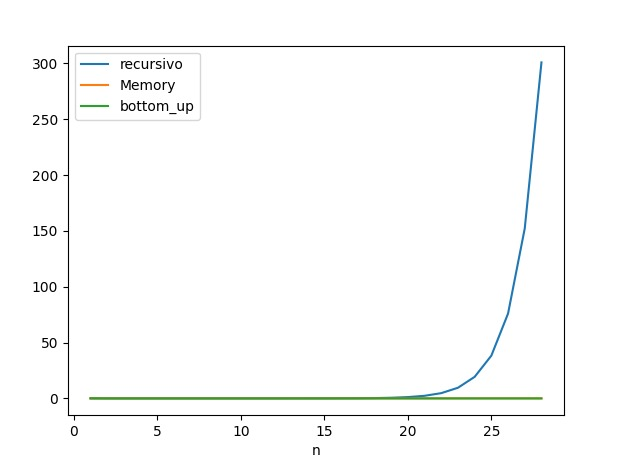
\includegraphics{GraficoAlgoritmos.jpg}
\caption{GraficoAlgoritmos}
\end{figure}

Después de realizar el análisis y la comparación entre los algoritmos
mediante la tabla y las gráficas obtenidas gracias a la librería
``pandas'' de Python, se puede apreciar claramente que los algoritmos
basados en memoria son significativamente mejores que el algoritmo
recursivo. Es importante destacar que, el algoritmo recursivo alcanza
valores exponencialmente superiores a partir de la iteración número 20.

\hypertarget{regresion-ols}{%
\subsection{Regresion OLS}\label{regresion-ols}}

En última instancia, es imprescindible realizar una comparación
exhaustiva entre la complejidad práctica calculada y la complejidad
teórica expresada como f(n). Para llevar a cabo este análisis, se
empleará la librería de Python denominada ``statsmodels'', gracias a la
cual podremos contrastar los resultados tabulados con la función de
complejidad mediante la aplicación de una regresión OLS (regresión por
mínimos cuadrados ordinarios). Esta herramienta matemática cuenta con
dos indicadores clave que nos permitirán evaluar la calidad del ajuste
obtenido. El primero de ellos es el coeficiente de determinación,
también conocido como R-squared, el cual adopta valores entre 0 y 1.
Cuanto más cercano sea este valor a 1, mayor será el grado de ajuste
proporcionado por la regresión. Por otro lado, el segundo indicador que
se utilizará es el coeficiente de correlación, cuyo cálculo se basa en
la relación existente entre dos variables. De esta forma, su análisis
permitirá obtener un valor preciso del tiempo requerido para un valor
dado de n.

\hypertarget{recursivo}{%
\subsubsection{Recursivo}\label{recursivo}}

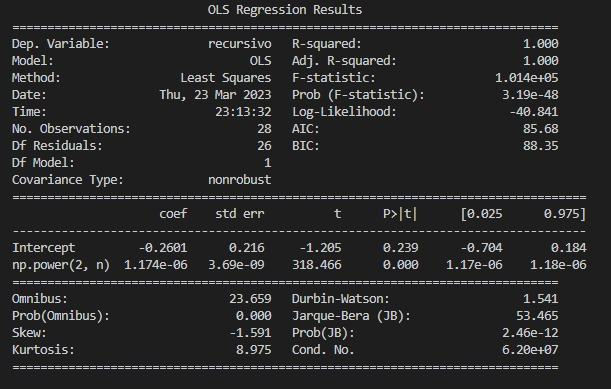
\includegraphics{OLSTABLA1.jpg} 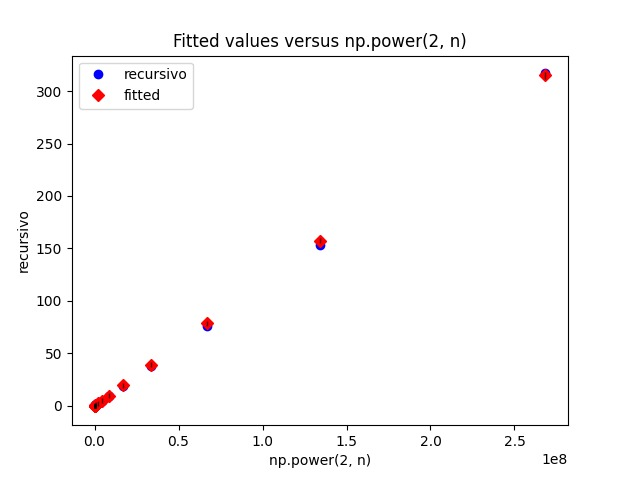
\includegraphics{OLSGRAFICO1.jpg}

La tabla presentada muestra los resultados de la regresión OLS aplicada
a los datos tabulados del algoritmo recursivo. El valor R-squared, que
representa el coeficiente de determinación, tiene un valor de 1.000, lo
que indica que la dispersión observada en los datos se ajusta
perfectamente a la complejidad identificada. Además, el coeficiente
denominado como coef tiene un valor de 1.174 × 10−6, lo que permite
establecer una relación exacta entre ambos factores.

Por lo tanto, se puede afirmar que la ecuación del tiempo dado n
elementos está correctamente representada por la regresión OLS obtenida
a partir de los datos tabulados del algoritmo recursivo. En
consecuencia, esta ecuación puede ser utilizada para predecir el tiempo
requerido para ejecutar el algoritmo en función del número de elementos
que se estén procesando.

\hypertarget{memorizado}{%
\subsubsection{Memorizado}\label{memorizado}}

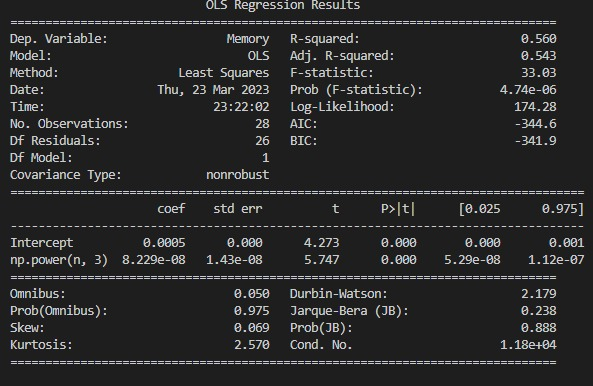
\includegraphics{OLSTABLA2.jpg} 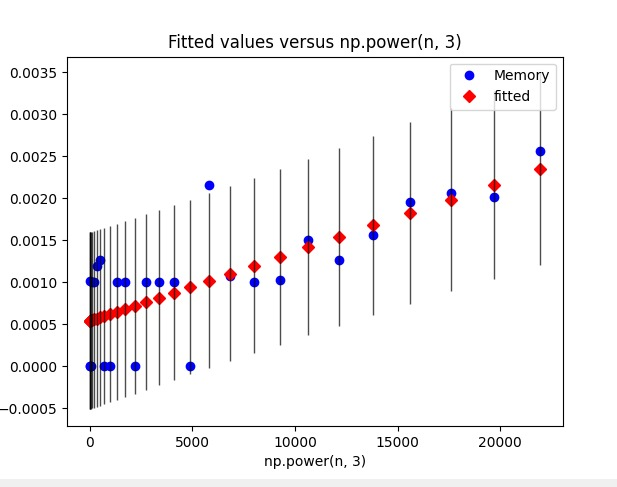
\includegraphics{OLSGRAFICO2.jpg}

En la tabla presentada se muestran los resultados de la regresión OLS
aplicada a los datos tabulados del algoritmo implementado. El valor
R-squared, que representa el coeficiente de determinación, es de 0.560,
lo que indica que la dispersión observada en los datos tiene una
relación positiva con la complejidad identificada. Además, el
coeficiente denominado como `coef' tiene un valor de 8.229 × 10−8, lo
que permite establecer una relación entre el tiempo requerido para
ejecutar el algoritmo y el número de elementos que se están procesando.

Así pues, se puede afirmar que la ecuación del tiempo dado n elementos
está correctamente representada por la regresión OLS obtenida a partir
de los datos tabulados del algoritmo implementado. En consecuencia, esta
ecuación puede ser utilizada para predecir el tiempo requerido para
ejecutar el algoritmo en función del número de elementos que se estén
procesando.

\hypertarget{tabulado}{%
\subsubsection{Tabulado}\label{tabulado}}

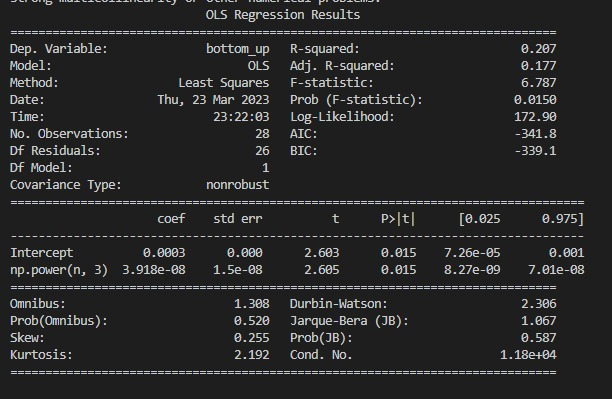
\includegraphics{OLSTABLA3.jpg} 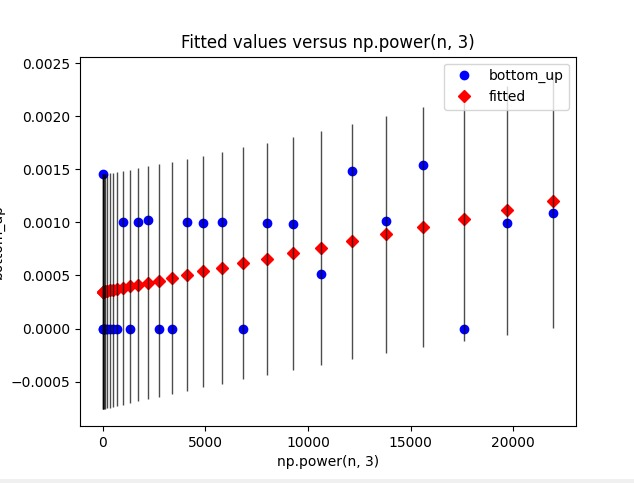
\includegraphics{OLSGRAFICO3.jpg}

El valor de R-squared obtenido es de 0.207, lo que indica que el modelo
de regresión utilizado explica únicamente un 20.7\% de la variabilidad
de la variable dependiente en función de la variable independiente. El
valor del coeficiente de regresión denominado `coef' es 3.918e-08, lo
que sugiere una relación muy débil entre las variables. Se puede
observar que tanto el intercepto como la variable independiente tienen
valores significativos, lo que sugiere que ambos términos son
importantes para explicar la variabilidad de la variable dependiente. En
general, se podría afirmar que la relación entre las variables no es muy
fuerte y que el modelo utilizado no explica bien la variabilidad en la
variable dependiente, sin embargo la complejidad teorica si es la
presentada.

\pagebreak
\hypertarget{parte-4}{%
\section{Parte 4}\label{parte-4}}

\hypertarget{pruebas-unitarias}{%
\subsection{Pruebas Unitarias}\label{pruebas-unitarias}}

Las pruebas unitarias son una técnica de programación que consiste en
realizar pruebas exhaustivas a un conjunto de funciones o métodos, de
manera individual y controlada, con el objetivo de verificar el correcto
funcionamiento del código, antes de ser implementado.

En el caso de los algoritmos dinámicos, estas pruebas son
particularmente importantes, ya que estos algoritmos utilizan técnicas
complejas y recursivas, donde es fácil caer en la generación de errores
sutiles que pueden llevar a resultados inconsistentes. A continuación se
presenta una breve explicación de cada prueba unitaria:

\begin{itemize}
\item
  test\_case\_0: se comprueba que el algoritmo implementado en las
  funciones \texttt{Recursive}, \texttt{Memory} y \texttt{BottomUp}
  retorna correctamente los valores para un caso base. En este caso, se
  utiliza una lista con un solo elemento.
\item
  test\_case\_1: se comprueba que el algoritmo implementado en las
  funciones \texttt{Recursive}, \texttt{Memory} y \texttt{BottomUp}
  retorna correctamente el valor máximo de una lista con dos elementos,
  uno de ellos negativo.
\item
  test\_case\_2: se comprueba que el algoritmo implementado en las
  funciones \texttt{Recursive}, \texttt{Memory} y \texttt{BottomUp}
  retorna correctamente una lista con tres elementos (dos de ellos
  negativos).
\item
  test\_case\_3: se comprueba que el algoritmo implementado en las
  funciones \texttt{Recursive}, \texttt{Memory} y \texttt{BottomUp}
  retorna correctamente una lista con cuatro elementos (uno de ellos
  negativo).
\item
  test\_case\_4: se comprueba que el algoritmo implementado en las
  funciones \texttt{Recursive}, \texttt{Memory} y \texttt{BottomUp}
  retorna correctamente una lista con cinco elementos (dos de ellos
  negativos).
\item
  test\_case\_5: se comprueba que el algoritmo implementado en las
  funciones \texttt{Recursive}, \texttt{Memory} y \texttt{BottomUp}
  retorna correctamente una lista con seis elementos (tres de ellos
  negativos).
\end{itemize}

Todas las pruebas fueron exitosas, lo que demuestra que las funciones
\texttt{Recursive}, \texttt{Memory} y \texttt{BottomUp} están
implementadas correctamente y devuelven los resultados esperados.

\hypertarget{parte-5}{%
\section{Parte 5}\label{parte-5}}
\pagebreak
\hypertarget{codigos-usados}{%
\subsection{Codigos usados}\label{codigos-usados}}

Todos los codigos usados se pueden encontrar dentro de la carpeta
Codigos presentada en este documento

    \begin{tcolorbox}[breakable, size=fbox, boxrule=1pt, pad at break*=1mm,colback=cellbackground, colframe=cellborder]
\prompt{In}{incolor}{ }{\boxspacing}
\begin{Verbatim}[commandchars=\\\{\}]

\end{Verbatim}
\end{tcolorbox}

\end{document}
